\documentclass{article}
\usepackage[utf8]{inputenc}
\usepackage[english]{babel}
\usepackage[margin=1in]{geometry}

\usepackage{fancyhdr}
\usepackage{extramarks}
\usepackage{amsmath}
\usepackage{amsthm}
\usepackage{amsfonts}
\usepackage{tikz}
\usepackage[plain]{algorithm}
\usepackage{algpseudocode}
\usepackage{arydshln}
\usepackage{mathtools}
\usepackage{cases}
\usepackage{listings}
\usepackage[numbered]{mcode}
\usepackage{booktabs}
\usepackage{graphicx}
\usepackage{subfigure}

\usepackage{blindtext}
\usepackage{amssymb}
\usepackage{hyperref}
\hypersetup{
    colorlinks=true,
    linkcolor=blue,
    filecolor=magenta,
    urlcolor=cyan,
}

\urlstyle{same}

%\newtheorem{theorem}{Theorem}
\newtheorem{theorem}{Theorem}[section]
\newtheorem{corollary}{Corollary}[theorem]
\newtheorem{lemma}[theorem]{Lemma}
\theoremstyle{remark}
\newtheorem*{remark}{Remark}

\theoremstyle{definition}
\newtheorem{definition}{Definition}[section]

\title{CS 250 - Computer Architecture \\ Extra Credit}
\author{Jincheng He Email: jincheng.he@dukekunshan.edu.cn}
\date{December 7, 2021}

\begin{document}

    \maketitle


    \section{spy1 program}
    First let me say the result, the password is: \textbf{spoon50303stocking!} and the secret is: \textbf{kind table}. As shown in figure~\ref{fig:spy1_result}.

    \begin{figure}[!htbp]
        \centering
        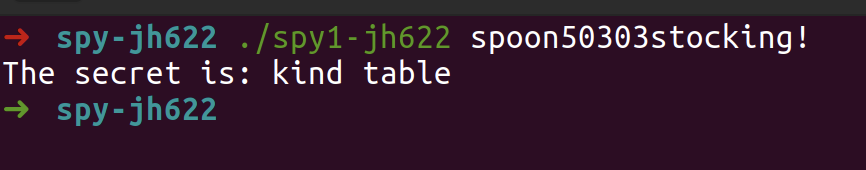
\includegraphics[width=0.6\textwidth]{img/spy1_result.png}
        \caption{spy 1 program result}
        \label{fig:spy1_result}
    \end{figure}

    Then I will talk about the process. First I use IDA to open the binary file, then I found figure~\ref{fig:spy1_decrypt}. Then I think it first decrypt the password by calling decrypt function, and then compare what I enter with this decrypted password. So I look into this decrypt function, and then by using the decompile feature in IDA, I found this in figure~\ref{fig:spy1_decrypt_func}.

    \begin{figure}[!htbp]
        \centering
        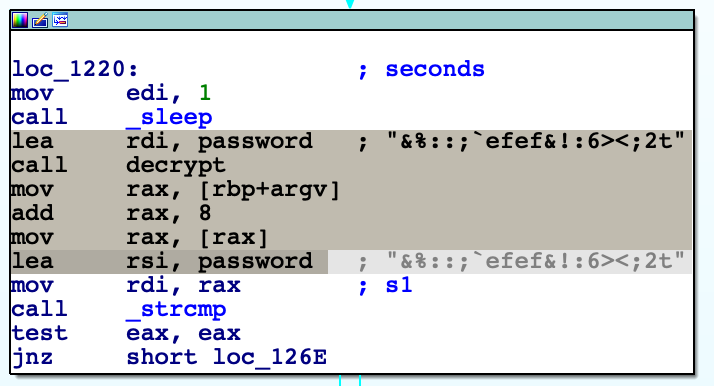
\includegraphics[width=0.6\textwidth]{img/ida_spy1_decrypt.png}
        \caption{ida screenshot}
        \label{fig:spy1_decrypt}
    \end{figure}

    \begin{figure}[!htbp]
        \centering
        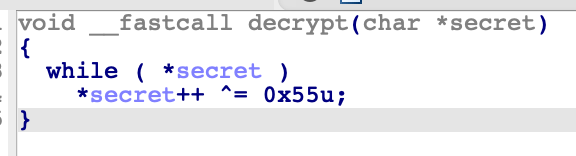
\includegraphics[width=0.6\textwidth]{img/spy1_decrypt_func.png}
        \caption{IDA decompile decrypt function}
        \label{fig:spy1_decrypt_func}
    \end{figure}

    So I wrote this program and get the password in figure~\ref{fig:spy1_myfunc}.

    \begin{figure}[!htbp]
        \centering
        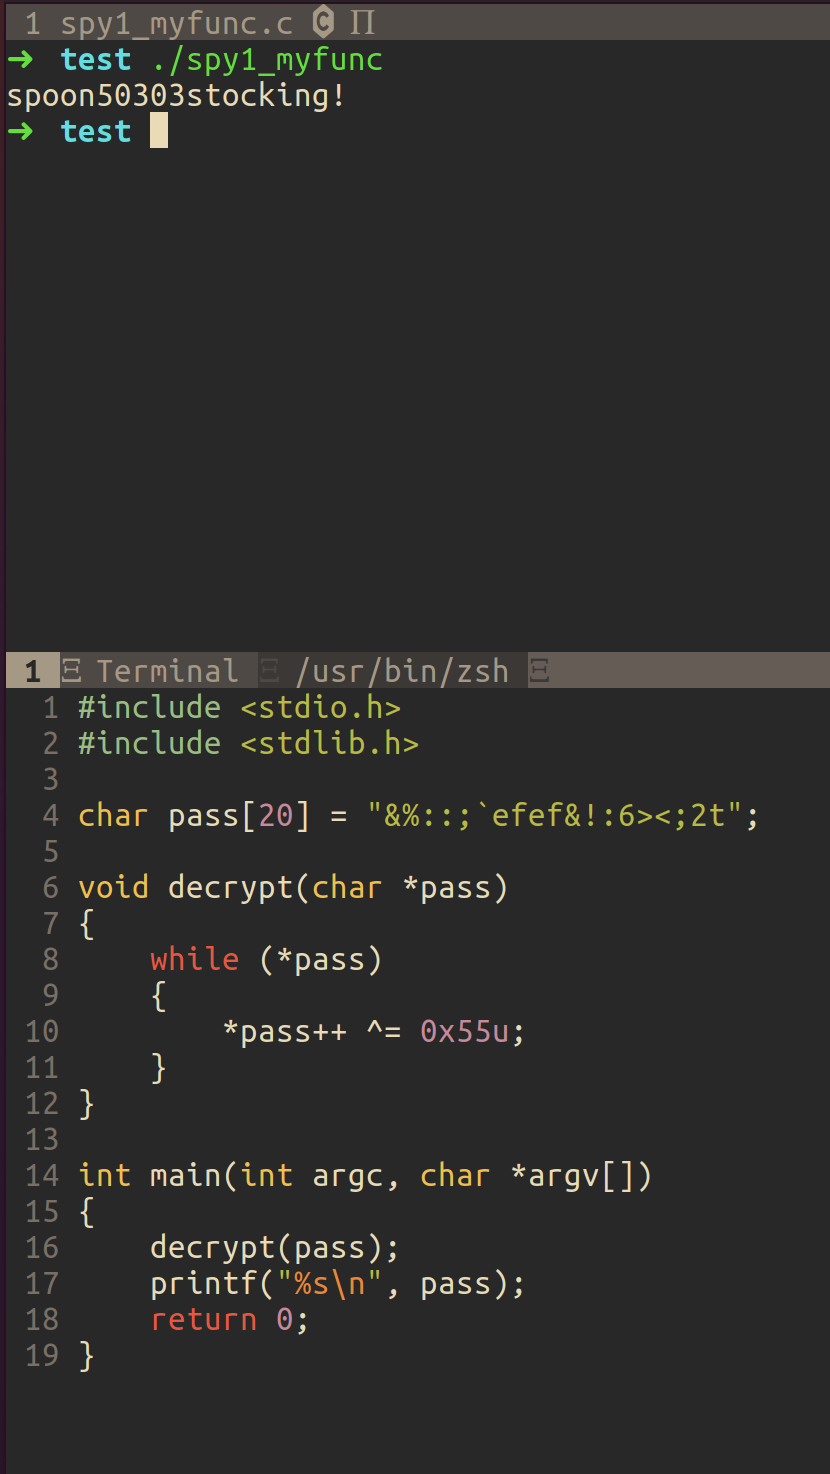
\includegraphics[width=0.4\textwidth]{img/spy1_myfunc.png}
        \caption{spy1 my function}
        \label{fig:spy1_myfunc}
    \end{figure}


    \section{spy2 program}
    For this problem, I only solved out the secret, which is: \textbf{material knot}. But I did not solve out the password. The idea of solving the secret is very similar to the spy 1. In figure~\ref{fig:spy2_secret}, I found out the secret, and need to be decrypted, this decrypt function is as same with the one in spy 1, so I wrote the program and the result is shown in figure~\ref{fig:spy_2_secret_result}. So the result of secret is: \textbf{material knot}.

    \begin{figure}[!htbp]
        \centering
        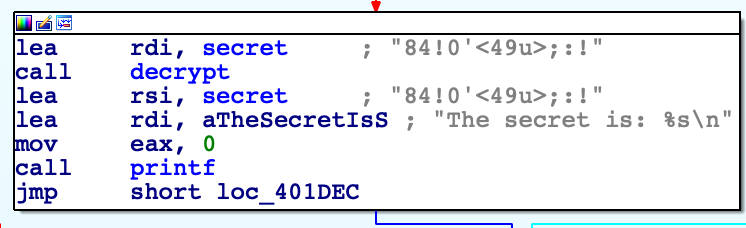
\includegraphics[width=0.6\textwidth]{img/spy2_secret.png}
        \caption{spy 2 secret screenshot}
        \label{fig:spy2_secret}
    \end{figure}

    \begin{figure}[!htbp]
        \centering
        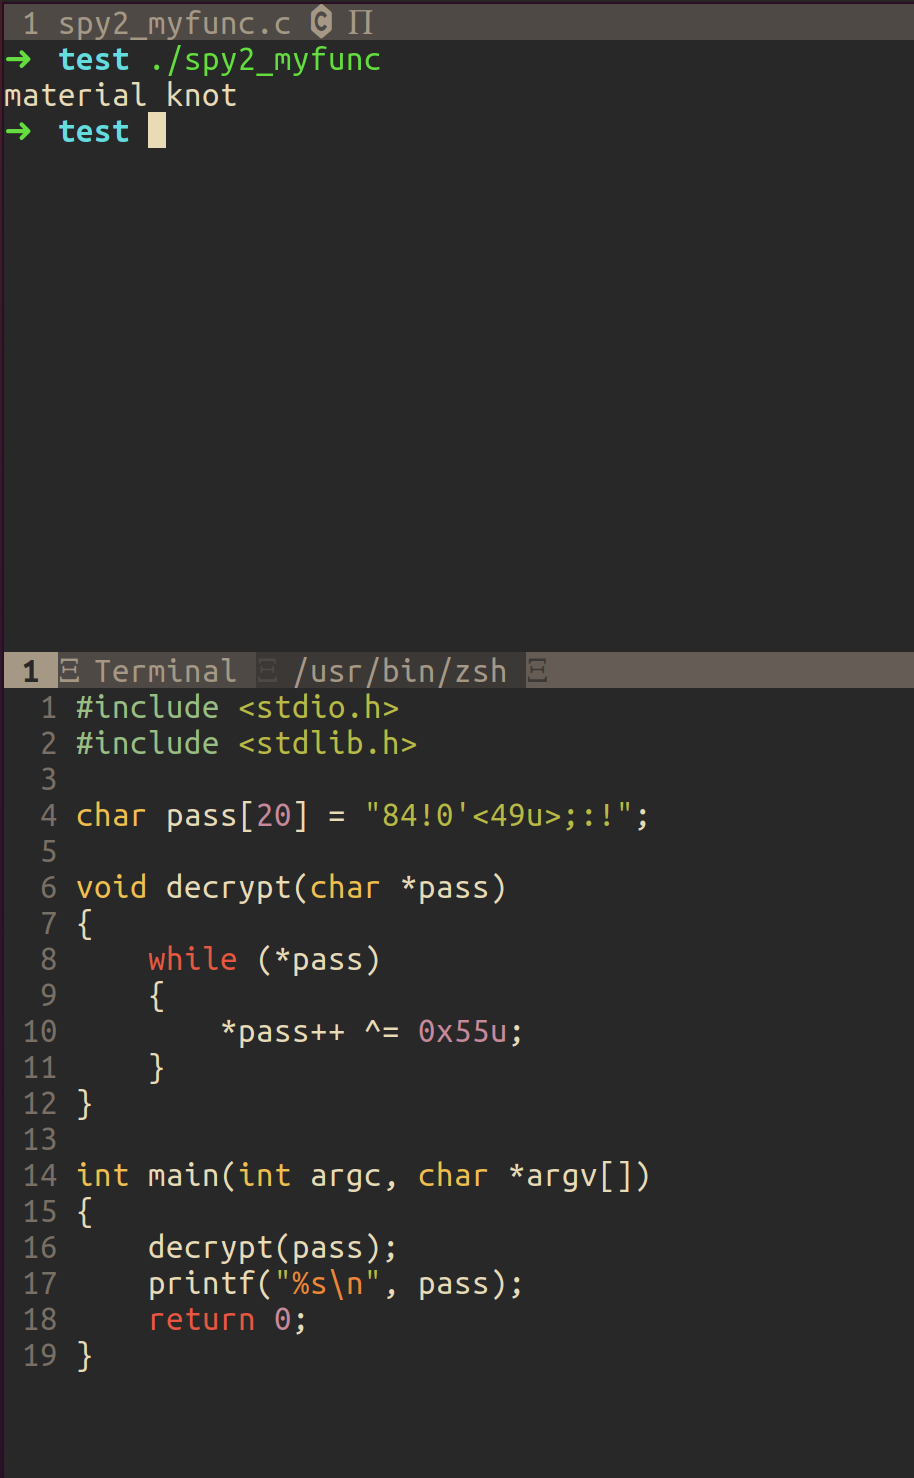
\includegraphics[width=0.5\textwidth]{img/spy2_secret_result.png}
        \caption{spy 2 program and result screenshot}
        \label{fig:spy_2_secret_result}
    \end{figure}


\end{document}